\chapter{2D LIDAR Feature Extraction for SLAM}
\label{cha:featureExtractor}

The exteroceptive sensors on the \imp, described in Chapter \ref{cha:Platform } are the Hokuyo Laser range finder and the 5 MP camera. In this thesis, the Hokuyo LIDAR output (i.e.,\ range data) is only utilized for feature extraction in SLAM. The feature detection algorithms extract either point features or linear features. 

\section{Feature Extraction with Point Features}
\label{sec:spike}
\subsection{Overview}
A point feature can be completely defined by its position in the inertial frame. In this section, a simplistic algorithm is described that could be used to detect point features in the environment. The algorithm is mainly based on large jumps in the range measurements of the LIDAR. The drawbacks of such an algorithm are discussed and improvements using preexisting knowledge of the environment are suggested.

\subsection{Feature Extraction Algorithm}
\label{sec: spikeAlgo}

To test the algorithm, a graphical simulation is built using V-REP\cite{vrep}. A simple environment is set up with four walls and a few cylinders to represent point features. The environment within the four walls is referred to as the arena and is shown in Figure~\ref{fig:3d_vrep}. In the simulated arena of Figure~\ref{fig:3d_vrep} the important aspects to observe are that, the entire arena is within the range of the LIDAR, and also the cylinders placed to represent point features are all relatively away from the wall. In such an environment, the distance readings gradually increase and decrease all along the walls except when they encounter an obstacle or a \textit{feature} resulting in the larger jumps in the distance readings that our algorithm looks for. The gradual change in the distance readings are more clearly seen when the scan values are plotted as a function of the angle of the scan beam with respect to the robot as shown in Figure~\ref{fig:Vrep_plot}.

\begin{figure}[h!]
    \centering
    \begin{subfigure}[b]{0.3\textwidth}
    
	    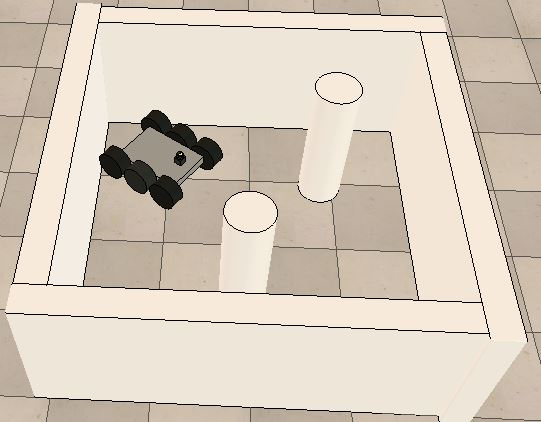
\includegraphics[width=\textwidth]{3d_vrep}
	    \caption{A simulated arena.}
	    \label{fig:3d_vrep}
    \end{subfigure}
    \quad %add desired spacing between images, e. g. ~, \quad, \qquad, \hfill etc.
      %(or a blank line to force the subFigure~onto a new line)
    \begin{subfigure}[b]{0.3\textwidth}
        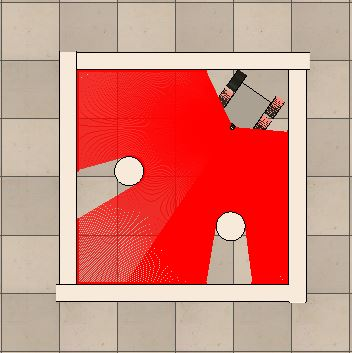
\includegraphics[width=\textwidth]{arena_vrep}
        \caption{Top view.}
        \label{fig:arena_vrep}
    \end{subfigure}%
        \caption{Simulated arena for LIDAR.}
        \label{fig:Simulated_1}
\end{figure}

For the robot to detect the large jumps, the distance is differentiated with respect to angles. As seen in Figure~\ref{fig:Vrep_cylinders}, this will give a specific pattern each time an obstacle (cylindrical in shape) is present. As outlined above,the feature detection may be achieved by considering the derivative of the range data. Namely, each time the derivative is larger than a fixed threshold and is a negative number, n object's beginning is found, and its end is found when a large positive value is encountered. Finding the midpoint of these two readings the location of the cylinder is found as in Figure~\ref{fig:Vrep_cylinders}. 
\begin{figure}
        \centering

        \begin{subfigure}[b]{0.48\textwidth}
                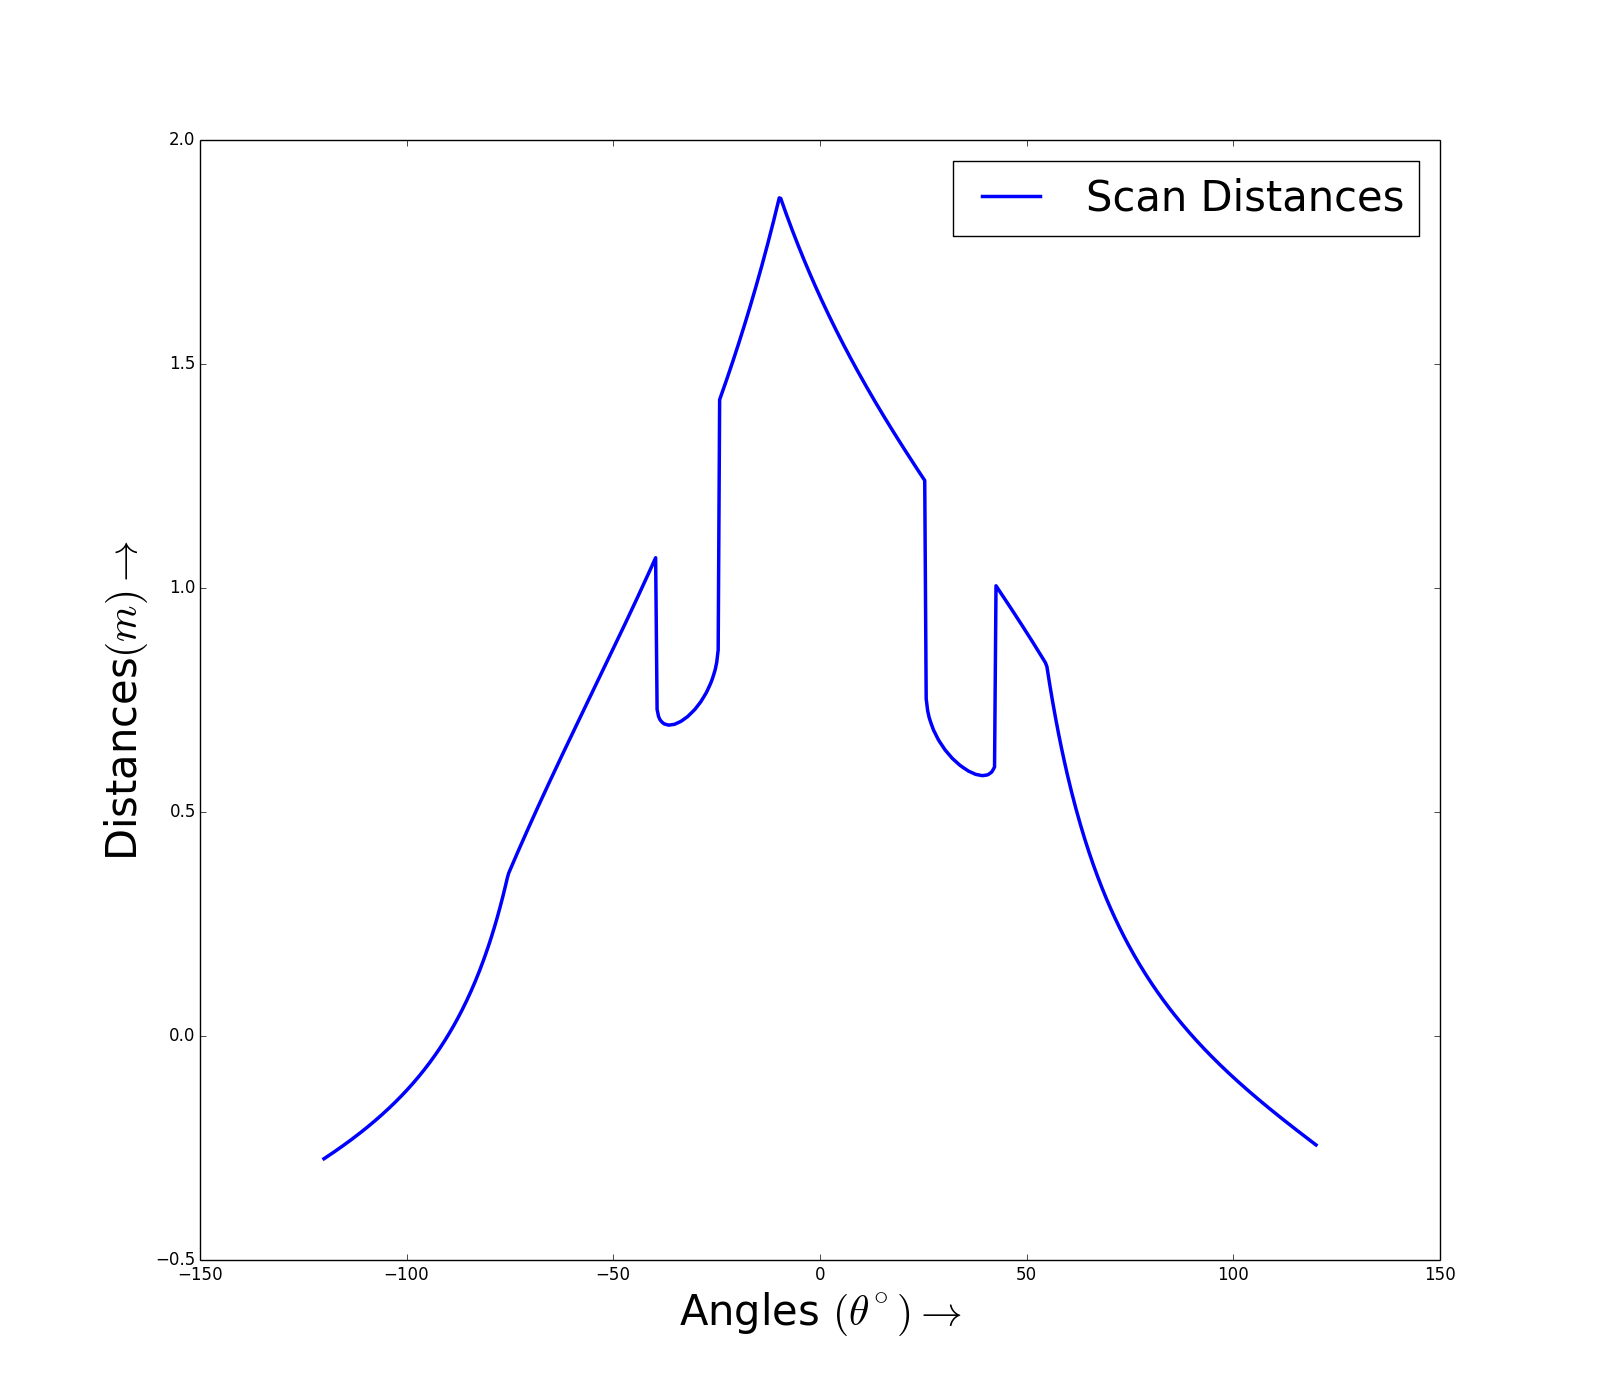
\includegraphics[width=\textwidth]{Vrep_plot}
                \caption{LIDAR scan.}
                \label{fig:Vrep_plot}
        \end{subfigure}
        \quad
        \begin{subfigure}[b]{0.48\textwidth}
                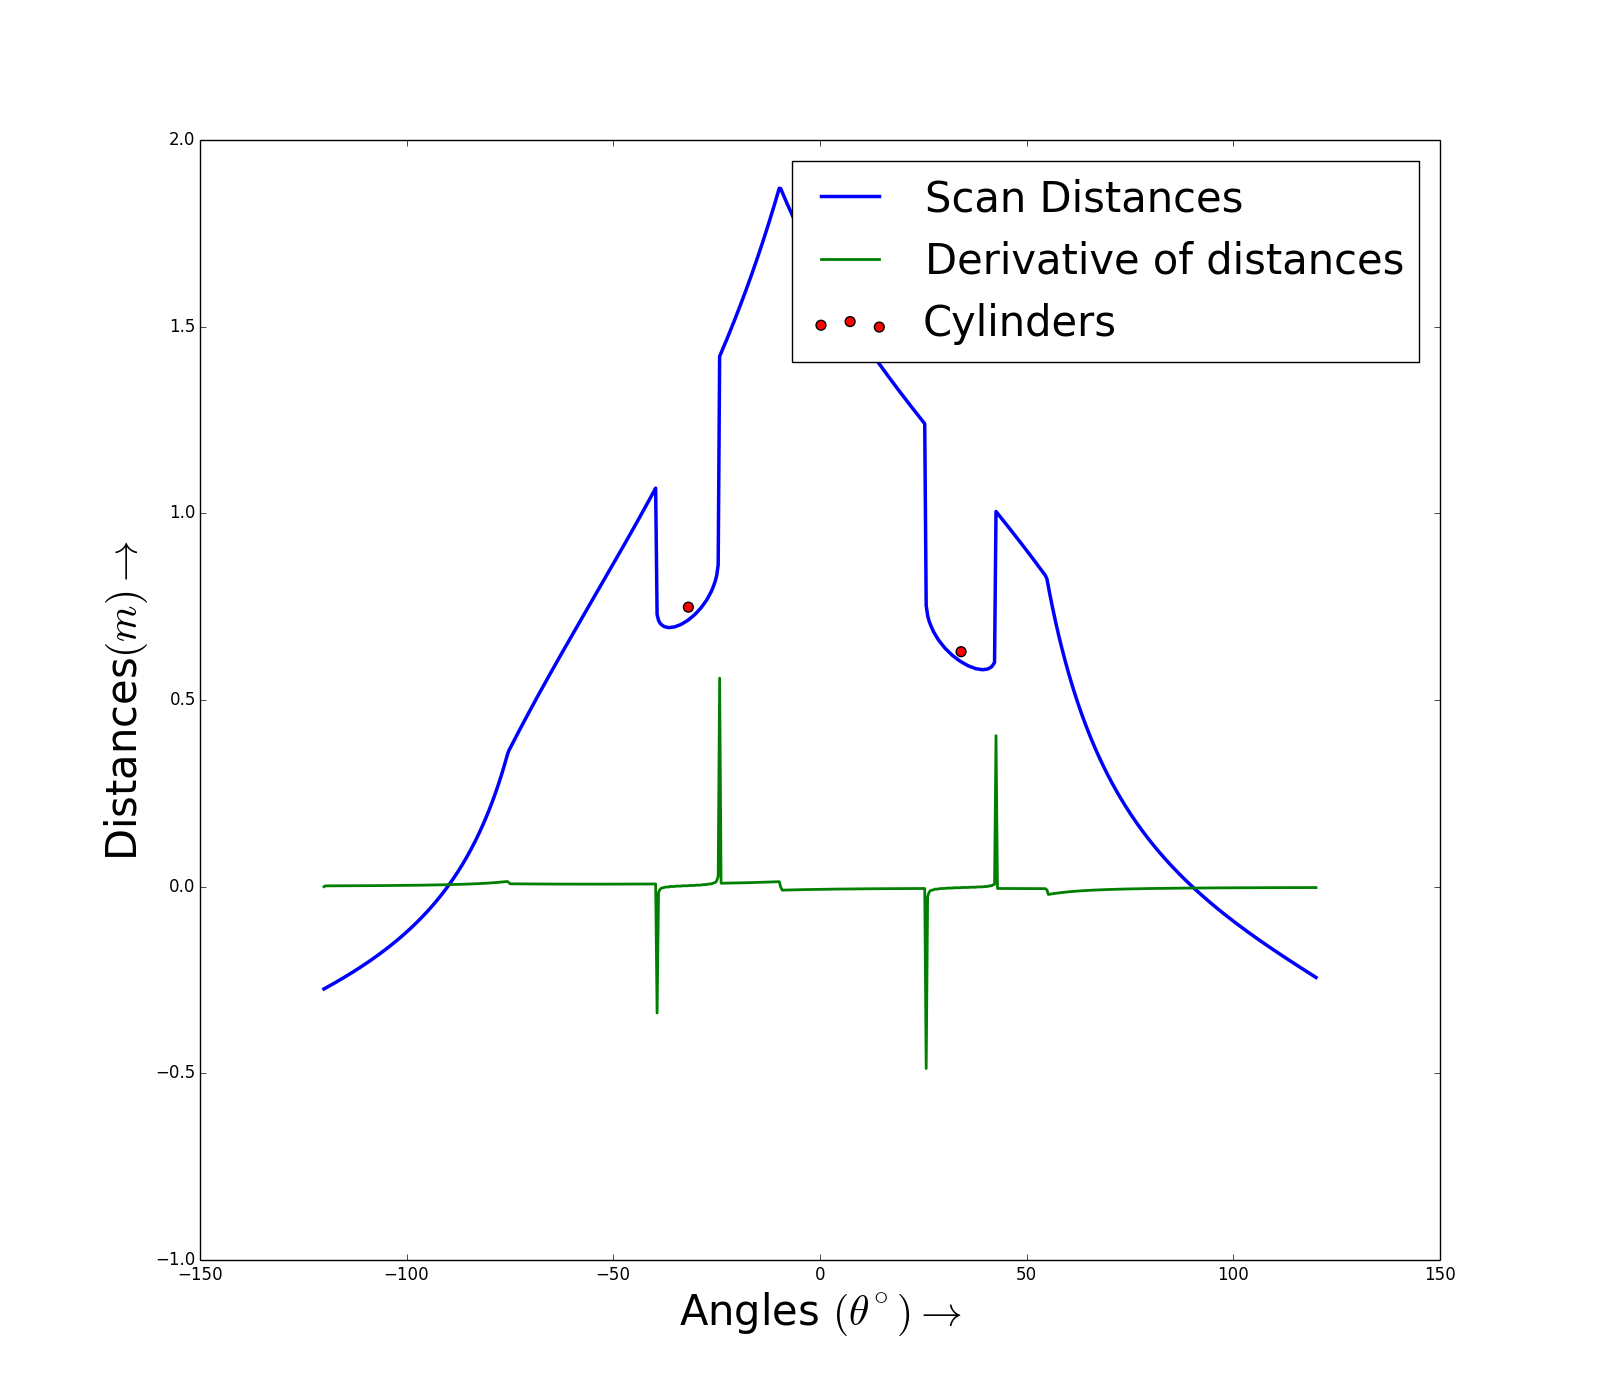
\includegraphics[width=\textwidth]{Vrep_cylinders}
                \caption{Detected cylinders.}
                \label{fig:Vrep_cylinders}
        \end{subfigure}

        \caption{Differential based LIDAR feature detection.}
        \label{fig:Simulated_2}
\end{figure}

It is apparent that this method has a large number of drawbacks. For example, if the arena is larger than the range of the LIDAR. At the points that the distance to any surface is greater than the LIDAR range, a zero value is returned. Leaving these values as zero, will introduce breaks in the range data which will have a detrimental affect on extracting features using the method of differentials outlined above. Another drawback is when there is an obstacle placed very close to a wall. The change in differentials corresponding to the obstacle are much smaller than the change corresponding to other landmarks. Reducing the threshold of differential jump will result in any small features of the arena such as doors being classified as obstacles. Hence it is seen, the choice of threshold for the change in derivative is a very sensitive tuning factor. 

To overcome the above shortcomings, a filter can be designed based on preexisting knowledge of the nature of features. A low threshold is set for the derivative of the range, which results in a large number of obstacles being detected. This set of obstacles is then thinned down by eliminating unlikely detections. Fist filter, is that all obstacles need to have a minimum number of non-zero LIDAR readings that lie on them. Based on the a priori known information, that the obstacle is in the shape of a cylinder with a known approximate radius, the approximate angular width that a prospective obstacle should occupy is predicted. The difference in the width of a candidate obstacle and the predicted width, can be used to remove a few prospective obstacles. There is still a chance of a segment of wall having the same angular width as the predicted width. This will result in spurious landmarks, hence each of the prospective obstacles are compared to the least square fit line for the same points. If the points all fit largely along the line, then it is a segment of the walls and can be removed from the list of possible candidates. By this method, a small amount of robustness is added to a simplistic algorithm of feature detection. The results of such a filter when applied with EKF can be seen in Section~\ref{sec:Spike_results}.

Once the features are detected, the measurement model from the robot to these features need to be calculated to be used in \ekf SLAM.

%
%
%
%
%
%The arena has to be fully within the range of the sensor, if not there will be breaks in the distance curve that will generate spurious landmarks. This drawback can be easily overcome by creating a zero order hold for those regions. Also any disturbances in the boundaries will also generate spurious landmarks. The threshold for the derivative is a very sensitive tuning parameter. If it is set too high there is an increased chance of missing landmarks placed close to walls and if it is set low, there are a large number of spurious landmarks. 
%
%To overcome this, based on preexisting knowledge of the nature of features a filter can be designed. A low threshold is chosen and a large number of prospective features are enumerated. All those that lack a minimum number of points on them are immediately eliminated. Next, based on the fact that the radius of the cylinders that are the landmarks is known, the angular width of any feature detected can be approximated. From the large set, only the ones within a range around this approximate angular width are retained. Then, the least squares fit is computed to check if the features are indeed cylinders or segments of the wall. Only the features having a large enough curvature are retained. 

\subsection{Examples and Validation on IMP}
\label{sec:Spike_results}

In a clean simulated arena, the efficacy of the first approach are seen in Section~\ref{sec: spikeAlgo}. But in a real world environment, a large number of variations will occur. To demonstrate this a relatively clean real world environment is considered as shown in Figure~\ref{fig:Real world arena}. 
\begin{figure}[h!]
    \centering
    \begin{subfigure}[b]{0.45\textwidth}
    
	    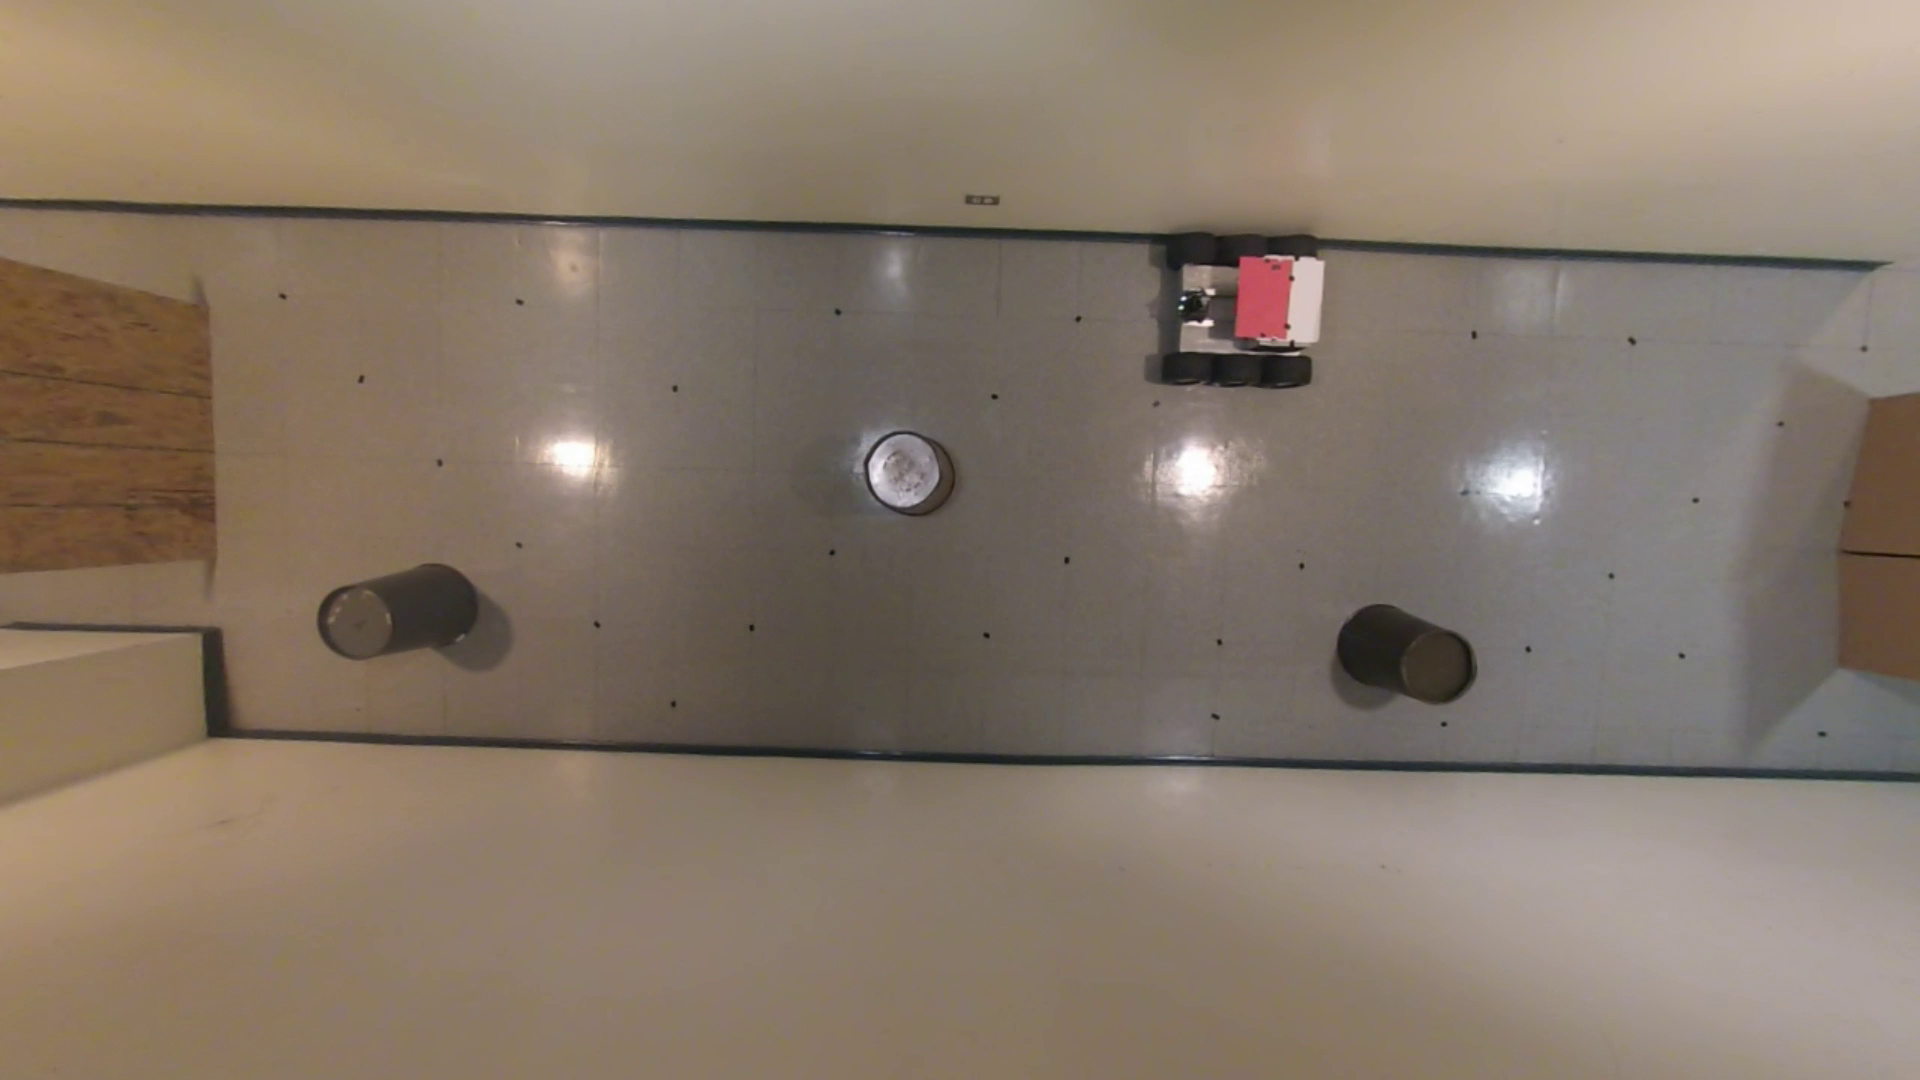
\includegraphics[width=\textwidth]{overhead}
	    \caption{Overhead view.}
	    \label{fig:overhead}
    \end{subfigure}
    \quad %add desired spacing between images, e. g. ~, \quad, \qquad, \hfill etc.
      %(or a blank line to force the subFigure~onto a new line)
    \begin{subfigure}[b]{0.45\textwidth}
        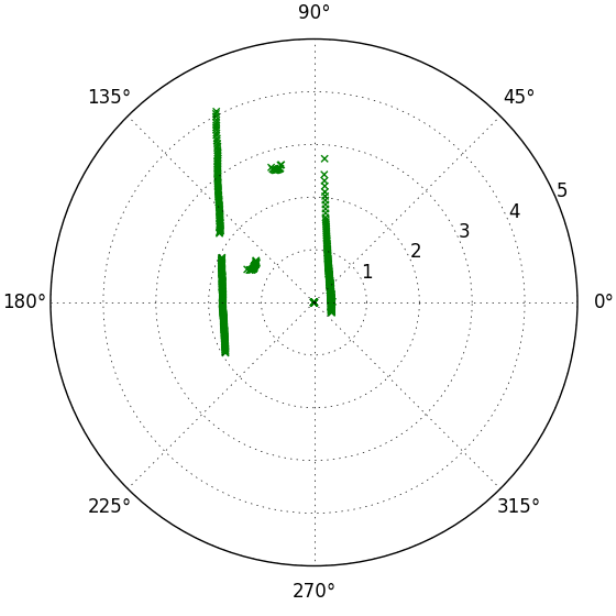
\includegraphics[width=\textwidth]{blank_scan}
        \caption{Polar plot of laser scan.}
        \label{fig:spike_scan}
    \end{subfigure}%
        \caption{Real world arena.}
        \label{fig:Real world arena}
\end{figure}

With such an arena, the simplistic approach of changes in derivatives being obstacles is tried with multiple threshold values.Even in the best case, out of the two obstacles within the range of the LIDAR, only one obstacle gets identified correctly. The other three obstacles detected are incorrect as seen in Figure~\ref{fig:Spike_cylinders_bad}.  

\begin{figure}[h!]
    \centering
    \begin{subfigure}[b]{0.45\textwidth}
	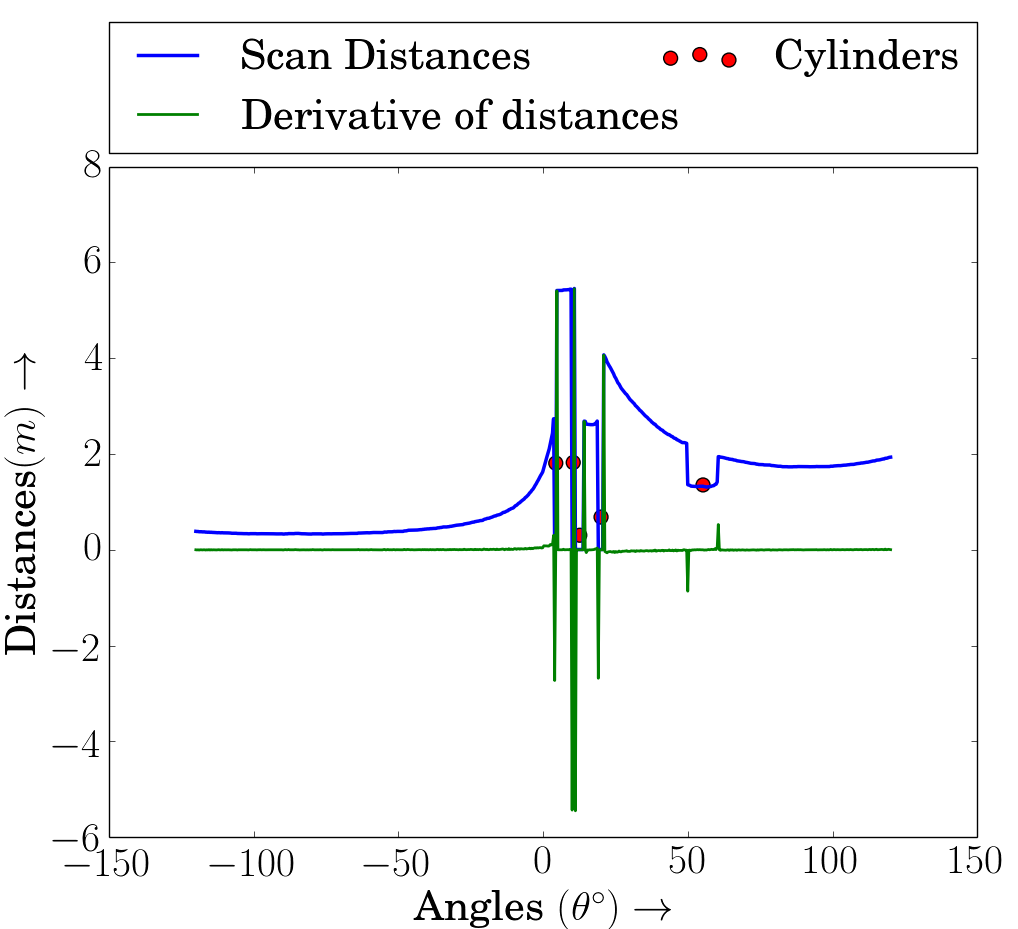
\includegraphics[width=\textwidth]{spike_cyl_bad}
    \end{subfigure}
    \quad %add desired spacing between images, e. g. ~, \quad, \qquad, \hfill etc.
      %(or a blank line to force the subFigure~onto a new line)
    \begin{subfigure}[b]{0.45\textwidth}
        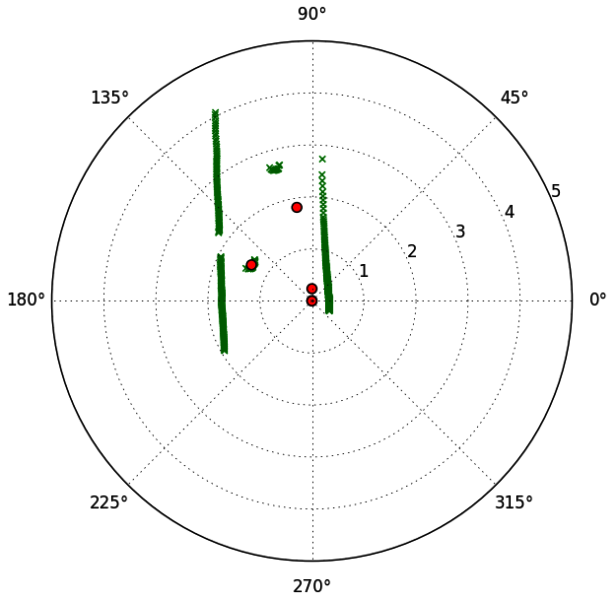
\includegraphics[width=\textwidth]{spike_cyl_badPol}
    \end{subfigure}%
	\caption{Spurious cylinders detected in data.}
	\label{fig:Spike_cylinders_bad}
\end{figure}

\begin{figure}[h!]
\centering
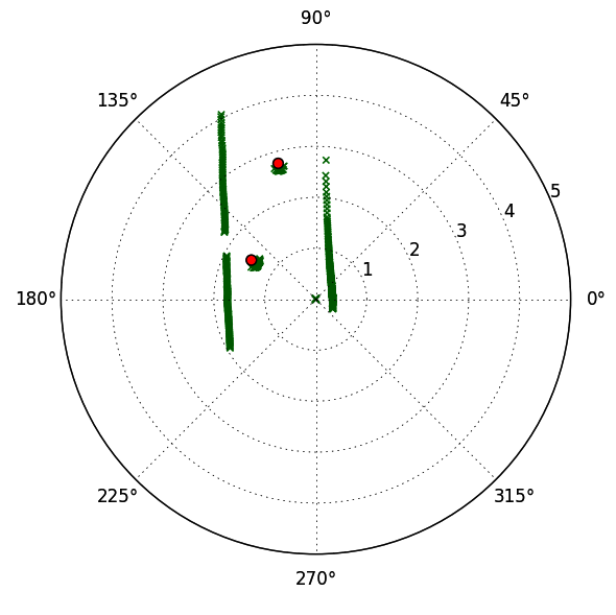
\includegraphics[width=0.4\textwidth]{spike_good}
\caption{After filtering of candidate cylinders.}
\label{fig:spike_good}
\end{figure}

To refine this, conditions similar to those discussed in section \ref{sec: spikeAlgo} are implemented. This is seen to give much better results. as seen in Figure~\ref{fig:spike_good}. 



\subsection{Measurement Model and the Corresponding Jacobian Matrices}
\label{sec:Spike_math}

Once an object's coordinates are found in the LIDAR data, its position has to be stored in the map.  Since an estimate of the robot's position in the inertial frame is known, the object coordinates are mapped from robot to inertial frame using a homogeneous transformation in 2 dimensions as shown in Equation~\ref{eq:SpikeMath1}:
\begin{equation}
\begin{bmatrix}
x_w\\y_w\\1
\end{bmatrix}=
\begin{bmatrix}
\cos(\theta_r) & -\sin(\theta_r) & x_r\\
\cos(\theta_r) & \sin(\theta_r) & y_r\\
0 & 0 & 1
\end{bmatrix}
\begin{bmatrix}
x_1\\y_1\\1
\end{bmatrix}
\label{eq:SpikeMath1}
\end{equation}
where, $ (x_w,y_w) $ are coordinates in the world frame,while $ (x_r,y_r,\theta_r) $ are the estimated pose of the robot and $ (x_1,y_1) $ are the object coordinates in the LIDAR frame.

For, data association, i.e.\ to check if the detected object is being seen for the first time or is being reobserved, the Euclidean distance is used. The euclidean distance between the detected object and the existing object positions is measured and if it is less than a particular threshold then the new object is associated with the existing one. 

For the correction of the robot pose as explained in section \ref{sec:EKF_SLAM}, the measurement model of the point features is needed. This is a mapping that gives the laser reading (i.e.\ range $ r $ and bearing $ \alpha $) from the robot to the object given by Equation \ref{eq:SpikeMath2}:
\begin{equation}
	\label{eq:SpikeMath2}
	h=\begin{bmatrix}
	r\\\alpha
	\end{bmatrix}=
	\begin{bmatrix}
	\sqrt{(y_1-y_r)^2+(x_1-x_r)^2} \\
	\tan^{-1}\left(\frac{y_1-y_r}{x_1-x_r}\right)-\theta_r.
	\end{bmatrix}
\end{equation} 

Using Equation \ref{eq:SpikeMath2} for both the existing landmarks and detected landmarks which have been expressed in the inertial frame, the \textit{innovation} from  Equation~\ref{eq:EKF_8} can be calculated. 

%
%
% the coordinates of the point feature in the robot's frame of reference are found using the inverse of the homogeneous transformation in Equation~\ref{eq:SpikeMath1}. But the robot pose used now is the new position at this particular time step. Once $ (x_1,y_1) $ is found in the robot frame, the measurement h can be found using Equation~\ref{eq:SpikeMath2}. The same equations are used for every corresponding feature that is detected to give $ z $ which is used to calculate the \textit{innovation} in Equation~\ref{eq:EKF_8}.


For the Kalman gain, according to Equation~\ref{eq:EKF_7} the derivatives of the model with respect to the state vector $ x \in \Re^n $ are used. The state contains both the robot pose and all the landmarks already existing in the map at that particular time step. Since it is assumed each landmark is independent of the other, most part of the Jacobian $ H $ contains zeros except for the part corresponding to the robot pose; if the measurement has been associated with an existing landmark, then it will also depend on that landmark's position. Hence for the Jacobian $ H $, the measurement model $ h $ is differentiated as follows:

\begin{equation}
\label{eq:SpikeMath3}
	H = 
	\begin{bmatrix}
	\frac{\partial r}{\partial x_r} & \frac{\partial r}{\partial y_r} & \frac{\partial r}{\partial \theta_r} & \cdots & \frac{\partial r}{\partial x_1} & \frac{\partial r}{\partial y_1} & \cdots \\
	\frac{\partial \alpha}{\partial x_r} & \frac{\partial \alpha}{\partial y_r} & \frac{\partial \alpha}{\partial \theta_r} & \cdots & \frac{\partial \alpha}{\partial x_1} & \frac{\partial \alpha}{\partial y_1} & \cdots 
	\end{bmatrix}.
\end{equation}

Each of the terms in H are derived separately as:


    \begin{equation}
	\frac{\partial r}{\partial x_r} = \frac{(x_r-x_1)}{\sqrt{(y_1-y_r)^2+(x_1-x_r)^2}} \qquad
	\frac{\partial \alpha}{\partial x_r} =  
	\frac{(y_1-y_r)}{(y_1-y_r)^2+(x_1-x_r)^2}
    \end{equation}
	\begin{equation}
    \frac{\partial r}{\partial y_r} = \frac{(y_r-y_1)}{\sqrt{(y_1-y_r)^2+(x_1-x_r)^2}} \qquad
	\frac{\partial \alpha}{\partial y_r} =  
	\frac{(y_r-y_1)}{(y_1-y_r)^2+(x_1-x_r)^2} 
    \end{equation}
	\begin{equation}
    \frac{\partial r}{\partial \theta_r} = 0 \qquad  
	\frac{\partial \alpha}{\partial \theta_r} = -1
    \end{equation}
	\begin{equation}
    \frac{\partial r}{\partial x_1} = \frac{(x_r-x_1)}{\sqrt{(y_1-y_r)^2+(x_1-x_r)^2}} \qquad
	\frac{\partial \alpha}{\partial y_1} =  
	\frac{(y_1-y_r)}{(y_1-y_r)^2+(x_1-x_r)^2} 
    \end{equation}
	\begin{equation}
    \frac{\partial r}{\partial x_1} = \frac{(y_r-y_1)}{\sqrt{(y_1-y_r)^2+(x_1-x_r)^2}} \qquad
	\frac{\partial \alpha}{\partial y_1} =  
	\frac{(y_r-y_1)}{(y_1-y_r)^2+(x_1-x_r)^2}.
    \end{equation}

The only other information needed for Kalman gain calculation is the observer error $ V^TRV $ with V being the derivative of the measurement model with respect to noise. If all landmarks are assumed to be uniformly affected by noise, it is reasonable to approximate V to be an identity matrix. R, the covariance of measurement noise, is a diagonal matrix with one of the eigenvalues representing the error in distance measurement of the LIDAR and the other eigenvalue being the angle measurement.R is given by,
\begin{equation}
\label{eq:SpikeMath5}
R = 
\begin{bmatrix}
\sigma_r & 0 \\
0 & \sigma_\alpha
\end{bmatrix}.
\end{equation}

Using all the measurement model and Jacobian matrices, it is possible to correct the estimate of the robot pose while simultaneously correcting the position of the landmarks. The result of such a \slam  is seen in Section~\ref{cha:results}.